\documentclass[a4paper,11pt]{article}
\usepackage[utf8]{inputenc}
\usepackage[spanish]{babel}
\usepackage{setspace}
\usepackage{apalike}
\usepackage[pdftex]{graphicx}
\bibliographystyle{apalike}
\begin{document}
\title{\Huge Estimación de la edad a partir de restos esqueléticos}
\author{Guillermo Ramírez García}
\date{\today}
\maketitle
\newpage
\spacing{1.5}
\part{Introducción}
Esto se debe a que, en las primeras edades de la vida, los cambios óseos están mejor sistematizados, por tratarse de un periodo de desarrollo y, por tanto, de cambios continuos \cite{scheuer2004juvenile}.

Por otra parte, aunque pueden existir variaciones en el ritmo de crecimiento entre unas poblaciones y otras, el grado de variabilidad no es muy amplio, por lo que las estimaciones suelen ser bastante acertadas.

Para reconstruir los patrones de las sociedades del pasado se siguen los mismos fundamentos que utiliza la Demografía; la única diferencia es que, en estos casos, se trabaja con poblaciones muertas, por lo que datos relativos a curvas de mortalidad o estimaciones sobre esperanza media de vida al momento del nacimiento se realizan en intervalos de cinco años, mientras que en la actualidad se hacen de año en año.

En Antropología Forense, la estimación de la edad se aplica, por lo general, en restos óseos o en cadáveres en avanzado estado de descomposición, para estimar la edad que tenía una persona al morir, con el objeto de contribuir a su identificación; no obstante, también se utiliza de forma habitual en los subadultos para la estimación de la edad de personas vivas, con el objeto de ubicar a un individuo en un marco legal; por ejemplo, en casos de inmigración, infanticidio, pedofilia, etc.
            
La metodología empleada para la determinación de la edad en Antropología Física, está basada en la evaluación del estado de desarrollo de un esqueleto, o edad fisiológica, y la correspondencia de ésta con la edad cronológica; a continuación se definen cada una de ellas.
La metodología empleada para la determinación de la edad en Antropología Física, está basada en la evaluación del estado de desarrollo de un esqueleto, o edad fisiológica, y la correspondencia de ésta con la edad cronológica:
\begin{itemize}
\item {\bf Edad fisiológica:} es la edad que refleja el estado fisiológico de un individuo. Se define según criterios de maduración y desarrollo en individuos infantiles y a partir de la evaluación de signos degenerativos en indivudos adultos. En el contexto de la Antropología Física, la edad fisiológica distingue entre la “edad dental” y la “edad esquelética”.
\item {\bf Edad cronológica:} está únicamente determinada por la fecha de nacimiento y de defunción. En los casos de identificación forense, se dispondrá de este dato como parte de la información {\em antemortem} y será proporcionado por los familiares, o a partir de documentos oficiales; así mismo, en caso de conocerse, será el criterio empleado para ubicar al individuo de acuerdo a las diferentes edades de transición establecidas por la ley, condicionando así la aplicación de leyes y derechos.
\end{itemize}
Para poder estimar la edad de un individuo en el contexto de la Antropología Forense de una forma eficiente y responsable, ya sea a partir de unos restos óseos o en sujetos vivos, el antropólogo deberá poseer unos conocimientos específicos y amplios en las siguientes materias:
\begin{itemize}
\item Anatomía esquelética y dental, tanto infantil como adulta.
\item Rangos normales de variación humana, esqueléticos y dentales.
\item Rasgos patológicos que puedan afectar a la aplicación del método.
\item Experiencia en la manipulación de material osteológico.
\item Conocimiento actualizado y experiencia en la aplicación de las diferentes metodologías existentes.
\item Capacidad para evaluar los diferentes indicadores de edad y sus criterios estadísticos.
\end{itemize}

\part{Metodología}
\section{Conceptos importantes}
El grado de ajuste entre la edad cronológica y fisiológica que ofrece un determinado método, debe ser evaluado y cuantificado; además, debe incluir información detallada referente al margen de error Intra-observador e Inter-observador asumido. Por un lado, esto permitirá al antropólogo la elección correcta del método que más se ajuste a las circunstancias específicas de su estudio y, por otro lado, se trata de un valor que deberá ser incorporado en el informe antropológico como requisito indispensable cuando se trabaje en contextos forenses, ofreciendo el valor de la edad estimada como un intervalo de confianza y con una determinada probabilidad de acierto.
\subsection{Precisión y exactitud}
En ciencia, se emplean ambos conceptos para describir la relación entre un valor numérico estimado con su valor real correspondiente. En la temática que aquí se trata, equivale a la relación entre la edad estimada a partir de un determinado método y la edad real del individuo. Se trata de dos conceptos independientes que, en el lenguaje cotidiano, son empleados como sinónimos pero, cuando se emplean en un lenguaje técnico, ofrecen información muy diferente:
\begin{itemize}
\item {\bf La precisión} informa sobre la dispersión de los resultados obtenidos cuando se aplica un determinado método repetidas veces, sobre una misma población de individuos con características similares. En el caso de la estimación de la edad, informa sobre el margen de error asumido por dicho método, expresado en forma de intervalo de edad estimada, dentro del cual existe una determinada probabilidad de que esté representado el valor de la edad real. Cuanto más preciso sea un método, menor será el intervalo de edad estimada que ofrezca.
\item {\bf La exactitud} informa sobre la desviación del valor estimado por un determinado método con respecto al valor real. En el caso de la estimación de la edad, equivale a la probabilidad de que la edad real del individuo se encuentre dentro del intervalo de edad estimada ofrecida por el método.
\end{itemize}
Ambos conceptos dependen de factores diferentes, por lo que pueden ser utilizados de forma conjunta para informar sobre la aplicabilidad de un determinado método.
\begin{enumerate}
\item {\bf Método poco preciso y muy exacto:} en este caso, el intervalo de edad estimada sería muy amplio, no obstante, éste contendría la edad real con una probabilidad muy elevada. Esta situación podría producirse, por ejemplo, al emplear un método que fue diseñado, combinando la información de diversas poblaciones muy diferentes entre sí.
\begin{figure}[h!]
\centering
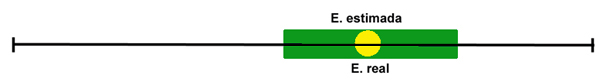
\includegraphics[scale=2]{1.jpg}
\end{figure}
\item {\bf Método poco preciso y poco exacto:} el intervalo de edad ofrecido sería muy pequeño; no obstante, la probabilidad de que la edad real se encontre dentro de dicho intervalo sería muy reducida. Este caso se produce, por ejemplo, cuando se aplican métodos que utilizan variables métricas muy precisas, pero que han empleado un volumen de muestra muy reducido para su diseño, por lo que no contemplan la variabilidad del rasgo analizado.
\begin{figure}[h!]
\centering
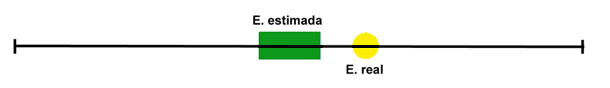
\includegraphics[scale=2]{2.jpg}
\end{figure}
\item {\bf Método muy preciso y muy exacto:} el intervalo de edad estimada es muy reducido y posee una gran probabilidad de incluir el valor de la edad real. Se trata de las características ideales que debe poseer un método para su aplicación en contextos forenses. Este caso se pude producir, por ejemplo, al emplear métodos que utilizaron grandes muestras de estudio para ser diseñados, que analicen variables métricas muy precisas y aplicados en la misma población que les dio origen.
\begin{figure}[h!]
\centering
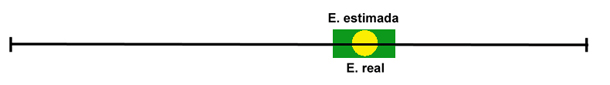
\includegraphics[scale=2]{3.jpg}
\end{figure}
\item {\bf Método poco preciso y poco exacto:} al contrario que el caso anterior, el intervalo de edad estimada es muy amplio y, además, existe una probabilidad reducida de que albergue la edad real. En este caso, podría mencionarse como ejemplo, un método que analice una variable débilmente relacionada con la edad del individuo.
\begin{figure}[h!]
\centering
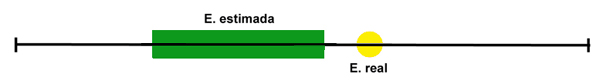
\includegraphics[scale=2]{4.jpg}
\end{figure}
\end{enumerate}

\subsection{Sensibilidad y especificidad}
En ocasiones, se emplean metodologías que no ofrecen como resultado un valor numérico, sino que informan sobre la posibilidad de que se cumpla, o no, una determinada condición, por lo que los únicos resultados posibles serán “sí” o “no”. En el contexto de la estimación de la edad, se trata de metodologías que evalúan determinados acontecimientos discretos en el proceso de maduración del esqueleto, para inferir si el individuo ha superado, o no, una edad concreta. Como ejemplos más destacados se pueden mencionar la unión de las epífisis de los huesos largos, la erupción dental, obliteración de las suturas craneales, etc.

En estos casos, los conceptos de sensibilidad y especificidad, se emplean para evaluar la validez del método, es decir, su capacidad para ubicar a cada individuo en su grupo de edad correspondiente, en función del resultado positivo, o negativo que se desprenda tras aplicar el método. Para explicar ambos conceptos se puede plantear como ejemplo la evaluación de un método antropológico cuyo objetivo es estimar si un individuo es mayor de edad, es decir, posee más de 18 años:
\begin{itemize}
\item {\bf Sensibilidad:} se define como la capacidad del método para detectar positivos, es decir, para identificar aquellos individuos que son mayores de 18 años.
\item {\bf Especificidad:} se define como la capacidad del método para detectar negativos, es decir, para identificar aquellos individuos que son menores de 18 años.
\end{itemize}
Aunque parezcan similares, ambos conceptos son complementarios y cada uno informa sobre una característica diferente del método. A continuación se muestran las 4 combinaciones posibles que se pueden realizar, empleando valores extremos, aplicadas al ejemplo anterior de un método cuyo fin es estimar la mayoría de edad:
\begin{enumerate}
\item {\bf Método muy sensible y muy específico:} posee una alta capacidad para detectar tanto positivos como negativos, por lo que es capaz de separar de manera muy eficiente a los individuos mayores de edad de los menores.
\begin{figure}[h!]
\centering
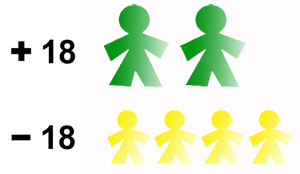
\includegraphics[scale=2]{5.jpg}
\end{figure}
\item {\bf Método muy sensible y poco específico:} alta capacidad para detectar positivos pero poca capacidad para detectar los negativos; es decir, clasifica de manera muy fiable a todos los individuos mayores de edad, pero es posible que también incluya como mayores de edad a individuos que no lo son, clasificando a estos como “falsos positivos”.
\begin{figure}[h!]
\centering
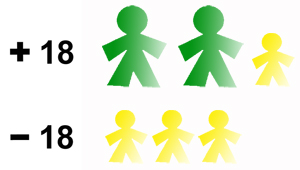
\includegraphics[scale=2]{6.jpg}
\end{figure}
\item {\bf Método poco sensible pero muy específico:} en este caso, posee poca capacidad de detectar positivos, pero alta capacidad para detectar a los negativos, es decir, no es un método muy fiable para detectar a los individuos mayores de edad, pero sí lo es para detectar a aquellos individuos que no lo son. Estos métodos tienen una elevada probabilidad de ofrecer “falsos negativos”.
\begin{figure}[h!]
\centering
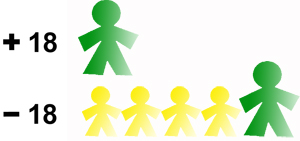
\includegraphics[scale=2]{7.jpg}
\end{figure}
\item {\bf Método poco sensible y poco específico:} posee poca capacidad para detectar tanto a los negativos como a los positivos, por lo que se trata de un método ineficaz para estimar la mayoría de edad.
\begin{figure}[h!]
\centering
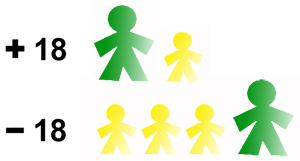
\includegraphics[scale=2]{8.jpg}
\end{figure}
\end{enumerate}
\newpage
\bibliography{Biblio}
\end{document}